\id{МРНТИ 31.23.39}{https://doi.org/10.58805/kazutb.v.4.25-441}

\begin{articleheader}
\sectionwithauthors{А.О. Сапиева, М.Г. Мурзагалиева, Н.С. Ашимхан, А.С. Зейнульдина, А.М. Габбасова, Ш.А. Мадиева, С.Б. Дюсекеева}{ИССЛЕДОВАНИЕ АНТИОКСИДАНТНОЙ И АНТИРАДИКАЛЬНОЙ АКТИВНОСТЕЙ
\emph{IN VITRO} ЭКСТРАКТОВ РАСТЕНИЙ, ПРОИЗРАСТАЮЩИХ НА ТЕРРИТОРИИ
КАЗАХСТАНА}

{\bfseries \textsuperscript{1}А.О. Сапиева, \textsuperscript{2}М.Г.
Мурзагалиева, \textsuperscript{2}Н.С. Ашимхан, \textsuperscript{1}А.С.
Зейнульдина,}

{\bfseries \textsuperscript{1}А.М. Габбасова,
\textsuperscript{1}Ш.А.Мадиева, \textsuperscript{1}С.Б.
Дюсекеева}\textsuperscript{\envelope }
\end{articleheader}

\begin{affiliation}
\textsuperscript{1}НАО «Медицинский университет Астана», Астана,
Казахстан,

\textsuperscript{2} КазНМУ им. С.Д. Асфендиярова, Алматы, Казахстан

\raggedright \textsuperscript{\envelope }Корреспондент-автор: \href{mailto:dyussekeyeva.s@amu.kz}{\nolinkurl{dyussekeyeva.s@amu.kz}}
\end{affiliation}

Данная работа посвящена сравнительному изучению содержания суммы
растворимых полифенольных соединений, антиоксидантной и антирадикальной
активностей экстрактов растений, произрастающих на территории Республики
Казахстан. Эксперименты \emph{in vitro} были проведены по общепринятой
методике определения общего содержания фенольных соединений методом
Фолина-Чокальтеу, общую антиоксидантную (восстановительную) активность
определяли методом железо - восстанавливающего потенциала (FRAP-метод),
антирадикальную активность методом ингибирования DPPH
(1,1-дифенил-2-пикрилгидразил) радикала анализируемыми веществами, с
использованием спектрофотометрических методов анализа. Анализ
совокупности полученных данных позволяет расположить исследуемые
экстракты в следующем ряду в зависимости от количества фенольных
соединений и значений антирадикальной и общей антиоксидантной
активностей экстрактов:
Гармала\textgreater Хвощ\textgreater Одуванчик\textgreater Солодка.

Выявлена выраженная положительная корреляция между содержанием фенольных
соединений и всеми показателями антиоксидантных свойств протестированных
фитопрепаратов. Среди исследуемых растений выделяются экстракты Гармалы
и Хвоща, как демонстрирующие наиболее высокий суммарный антиоксидантный
и антирадикальный потенциал. Представленные результаты являются основой
для дальнейшего более детального изучения антиоксидантных,
антирадикальных и гепатопротекторных свойств растительного
лекарственного сырья.

{\bfseries Ключевые слова:} антиоксидантная активность, антирадикальная
активность, полифенольные соединения, экстракты растений, \emph{in
vitro}, флавоноиды, спектрофотометрия.

\begin{articleheader}
{\bfseries ҚАЗАҚСТАН АЙМАҒЫНДА ӨСЕТІН ӨСІМДІК ЭКСТРАКТТАРЫНЫҢ
АНТИОКСИДАНТТЫ ЖӘНЕ АНТИРАДИКАЛЫҚ ҚЫЗМЕТІН IN VITRO ЗЕРТТЕУ}

{\bfseries \textsuperscript{1}А.О. Сапиева, \textsuperscript{2}М.Г.
Мурзагалиева, \textsuperscript{2}Н.С. Ашимхан, \textsuperscript{1}А.С.
Зейнульдина,}

{\bfseries \textsuperscript{1}А.М. Габбасова,
\textsuperscript{1}Ш.А.Мадиева, \textsuperscript{1}С.Б.
Дюсекеева}\textsuperscript{\envelope }
\end{articleheader}

\begin{affiliation}
\textsuperscript{1}КеАҚ «Астана медицина университеті», Астана,
Казахстан,

\textsuperscript{2} С.Д. Асфендияров атындағы КазҰМУ, Алматы, Казахстан,

e-mail: \href{mailto:dyussekeyeva.s@amu.kz}{\nolinkurl{dyussekeyeva.s@amu.kz}}
\end{affiliation}

Бұл жұмыс Қазақстан Республикасының аумағында өсетін өсімдік
сығындыларының еритін полифенолды қосылыстардың құрамын, антиоксиданттық
және антирадиалды белсенділігін салыстырмалы зерттеуге арналған. In
vitro эксперименттер фенолды қосылыстардың жалпы құрамын Фолин-Циокалтеу
әдісімен анықтаудың жалпы қабылданған әдісін қолдану арқылы жүргізілді,
жалпы антиоксиданттық (тотықсыздандырғыш) белсенділік темірді қалпына
келтіру потенциалы әдісімен (FRAP әдісі), антирадиалды белсенділік DPPH
тежеу әдісі (1,1-дифенил-2-пикрилгидразил) талдаудың
спектрофотометриялық әдістерін қолдана отырып, талданатын заттар бойынша
радикал. Алынған мәліметтердің жиынтық талдауы зерттелетін сығындыларды
фенолдық қосылыстардың мөлшеріне және сығындылардың антирадиалды және
жалпы антиоксиданттық белсенділіктерінің мәндеріне байланысты келесі
қатарға орналастыруға мүмкіндік береді:
Гармала\textgreater Жылқықұйрығы\textgreater Одуванчик\textgreater Мия.
Фенолдық қосылыстардың құрамы мен тексерілген шөптік препараттардың
антиоксиданттық қасиеттерінің барлық көрсеткіштері арасында айқын оң
корреляция анықталды. Зерттелген өсімдіктердің ішінде Хармала мен Жылқы
құйрығы сығындылары ең жоғары антиоксиданттық және антирадиалды әлеуетті
көрсететін ретінде ерекшеленеді. Ұсынылған нәтижелер өсімдік тектес
дәрілік шикізаттың антиоксиданттық, антирадиалды және гепатопротекторлық
қасиеттерін одан әрі егжей-тегжейлі зерттеуге негіз болып табылады.

{\bfseries Түйін сөздер:} антиоксиданттық белсенділік, антирадикалдық
белсенділік, полифенолды қосылыстар, өсімдік сығындылары, in vitro,
флавоноидтар, спектрофотометрия.

\begin{articleheader}
{\bfseries RESEARCH OF ANTIOXIDANT AND ANTIRADICAL ACTIVITIES \emph{IN
VITRO} OF EXTRACTS OF PLANTS GROWING ON THE TERRITORY OF KAZAKHSTAN}

{\bfseries \textsuperscript{1}А. Sapiyeva, \textsuperscript{2}M.
Murzagalieva, \textsuperscript{2}N. Ashimkhan, \textsuperscript{1}A.
Zeinuldina,} {\bfseries \textsuperscript{1}A. Gabbasova,}

{\bfseries \textsuperscript{1}Sh. Madiyeva, \textsuperscript{1}S.
Dyusekeeva}\textsuperscript{\envelope }
\end{articleheader}

\begin{affiliation}
\textsuperscript{1}Astana Medical University, Astana, Kazakhstan,

\textsuperscript{2}Asfendiyarov Kazakh National Medical University,
Almaty, Kazakhstan,

e-mail:
\href{mailto:dyussekeyeva.s@amu.kz}{\nolinkurl{dyussekeyeva.s@amu.kz}}
\end{affiliation}

This work is devoted to the comparative study of the content of the sum
of soluble polyphenolic compounds, antioxidant and antiradical
activities of plant extracts growing in the territory of the Republic of
Kazakhstan. In vitro experiments were carried out according to the
generally accepted method for determining the total content of phenolic
compounds by the Folin-Chocalteu method, the total antioxidant
(reducing) activity was determined by the method of iron-reducing
potential (FRAP method), antiradical activity by inhibition of the DPPH
(1,1-diphenyl-2-picrylhydrazyl) radical by the analyzed substances,
using spectrophotometric analysis methods. The analysis of the totality
of the data obtained allows us to place the studied extracts in the
following row, depending on the number of phenolic compounds and the
values of the antiradical and total antioxidant activities of the
extracts: Harmala\textgreater Equisetum\textgreater Taraxacum
\textgreater{} Liquorice.

A pronounced positive correlation was revealed between the content of
phenolic compounds and all indicators of the antioxidant properties of
the tested phytopreparations. Among the studied plants, extracts of
Harmala and Equisetum are distinguished as demonstrating the highest
total antioxidant and antiradical potential. The presented results are
the basis for further more detailed study of the antioxidant,
antiradical and hepatoprotective properties of herbal medicinal raw
materials.

{\bfseries Keywords}: antioxidant activity, antiradical activity,
polyphenolic compounds, plant extracts, in vitro, flavonoids,
spectrophotometry.

\begin{multicols}{2}
{\bfseries Введение.} Внимание исследователей в качестве объектов для
создания лекарственных средств привлекают природные соединения. В
настоящее время лекарственные препараты с антиоксидантной активностью
(АОА) широко используются в медицине для ингибирования процессов
перекисного окисления {[}1{]}. Известно, что в нормальных условиях
жизнедеятельности клетки постоянно присутствует определенный уровень
перекисного окисления липидов, индуцированный образованием активных форм
кислорода. Перекисное окисление липидов в клетке поддерживается на
постоянном уровне благодаря многоуровневой антиоксидантной системе
защиты {[}2{]}. Высокой антиоксидантной активностью характеризуются
аскорбиновая кислота, каротиноиды, вещества полифенольной природы,
которые содержатся в различных соотношениях в растительном сырье и их
экстрактах {[}3{]}. В природе есть более сильные антиоксиданты это,
флавоноиды и ароматические гидроксикислоты растительного происхождения.
Более 2 \% от общего количества органического углерода, полученного в
результате фотосинтеза в растениях, участвует в образовании флавоноидов
или других полифенолов {[}4{]}. Перспективы разработки новых и
эффективных фитопрепаратов связаны с поиском антиоксидантов, действующих
на данные процессы, поэтому поиск новых веществ с АОА во многих случаях
проводится в ряду флавоноидов, представляющих собой многочисленную
группу природных полифенолов. В настоящее время единичны случаи
применения отдельных флавоноидов, несмотря на их широкое разнообразие, а
также возобновляемость источников их получения. Выделение флавоноидов из
растительного сырья Казахстана с их последующей химической модификацией,
установление строения полученных производных и изучение их АОА в
настоящее время является весьма актуальным вопросом {[}5{]}.

Казахстан располагает уникальными запасами растений дикорастущих видов,
обладающих лекарственными свойствами, значительная часть которых
перспективна для исследований их химического состава и биологической
активности. В связи с этим очень актуальна задача разработки и внедрения
в производство фитопрепаратов и разработка научно-обоснованного
алгоритма рационального использования растительных богатств.

Как известно важным показателем биологической активности природных
соединений растительного происхождения является их разнообразие. В
первую очередь, это связано со структурным разнообразием природных
соединений, а также с тем, что каждое соединение способно воздействовать
на множество структурных и функциональных систем клетки и организма в
целом {[}6{]}. В настоящее время многие антиоксидантные и
гепатопротекторные препараты, применяемые в клинической практике,
являются синтетическими, вызывают аллергические реакции и обладают
выраженными кумулятивными свойствами. Именно это обстоятельство
обуславливает актуальность в фармакотерапии и профилактике заболеваний
"свободнорадикальной патологии" применение лекарственных средств
растительного происхождения, влияние которых вызвано синергизмом
действия таких основных классов природных соединений как полифенолы,
алкалоиды, аминофенолокислоты, витамины и другие вещества {[}7{]}. В
связи с вышеуказанным исследование антиоксидантной, антирадикальной и
гепатопротекторной активности веществ растительного происхождения, а
также определение возможности взаимосвязи между данными свойствами
приобретают актуальность и востребованность для медицины.

Как известно наиболее обширной группой фенольных соединений
растительного сырья являются флавоноиды. Большинство флавоноидов
оказывают на организм человека капилляроукрепляющее,
противовоспалительное и противоопухолевое действие {[}8{]}. Анализ
литературных сведений об исследуемых растениях показал, что одними из
основных биологически активных веществ, определяющих многие их
терапевтические свойства, являются фенольные соединения. Основу
комплексов составляют один или несколько классов фенольных соединений:
фенольные кислоты, фенилпропаноиды, флавоноиды, танины {[}9{]}.
Фенольные соединения -- одна из важнейших групп природных антиоксидантов
{[}10{]}. По своей активности они опережают такие мощные антиокислители,
как витамины C, E и бета-каротин. Появляется все больше доказательств их
протекторной активности в отношении множества неинфекционных заболеваний
человека.

\emph{Цель работы:} сравнительное изучение содержания суммы растворимых
полифенольных соединений, антиоксидантной (АОА) и антирадикальной
активностей экстрактов эндемичных растений Казахстана \emph{in vitro} с
помощью современных спектрофотометрических методов.

{\bfseries Материалы и методы:} Объектами исследования были выбраны водные
растительные экстракты солодки, хвоща, одуванчика и гармалы, широко
распространенных на территории Казахстана. В таблице 1 приведен
химический состав и полезные свойств данных растений.

Эксперименты \emph{in vitro} были проведены по общепринятой методике
Фолина-Чокальтеу, железо - восстанавливающего потенциала (FRAP) и
ингибированием DPPH (1,1-дифенил-2-пикрилгидразил) радикала
анализируемыми веществами с использованием спектрофотометрических
методов анализа.
\end{multicols}

\begin{longtable}[c]{|p{0.1\textwidth}|p{0.4\textwidth}|p{0.4\textwidth}|}
\caption*{Таблица 1- Химический состав и полезные свойства экстрактов
растений} \\
\hline
Растение &
  Химический состав надземной части в \% &
  Полезные свойства \\ \hline
\endfirsthead
%
\endhead
%
\begin{tabular}[c]{@{}l@{}}Хвощ\\   Equisetum\end{tabular} &
  алкалоиды (эквизетин, никотин, 3-метоксипиридин), сапонин эквизетонин, флавоноиды, органические кислоты (аконитовая, яблочная, щавелевая), жирное масло, эфирное масло, большое количество солей кремниевой кислоты, растворимых в органических соединениях, горечи, дубильные вещества, смолы и полиоксиантрахиноновые соединения. Найдены также небольшие количества аскорбиновой кислоты и каротина. &
  Мочегонное, кровоостанавливающее, противовоспалительное, способствует выведению свинца из организма. У животных с экспериментальным аллоксановым диабетом при введении 20\% настоя хвоща полевого снижается уровень глюкозы на 9,3\%. противовоспалительное, антимикробное, цитотоксическое действие. \\ \hline
\begin{tabular}[c]{@{}l@{}}Одуванчик\\   Taraxacum\end{tabular} &
  тритерпеновые соединения: тараксастерол, тараксерол, псевдотараксастерол, β-амирин; стерины: β-ситостерин, стигмастерин, тараксол; углеводы: до 40 \% инулина; жирное масло, в состав которого входят глицериды пальмитиновой, мелиссовой, линолевой, олеиновой, церотиновой кислот; каучук, белки &
  спазмолитическое, слабительное действие, повышают кислотность желудочного сока, противовоспалительное, противоопухолевое, гепатопротективное, антиатерсклеротическое, мочегонное, гипогликемическое, терапевтическое воздействие при гастритах и язвенной болезни желудка. \\ \hline
\begin{tabular}[c]{@{}l@{}}Гармала\\   Peganum\\ harmala\end{tabular} &
  алкалоиды, производные хиназолина и индола. В том числе –гармалин, гармин (банистерин), гармалол и L-пеганин (вазицин), пегамин, пеганол, дезоксипеганин, пеганидин (в траве) и др. &
  ингибирующее, противоопухолевое, антикоагулянтное, гипотензивное, антидиабетическое, антибактериальное, противовирусное, противовоспалительное, антипаразитарное, антидепрессантное, нейропротективное \\ \hline
\begin{tabular}[c]{@{}l@{}}Солодка\\   Glycyrrhí́za\\ glábra\end{tabular} &
  тритерпеновый сапонин глицирризин, флавоноиды, флавонолы, халконы, большое количество сахара, крахмала, слизи, аскорбиновой кислоты, стероидов, алкалоидов, эфирных масел, жироподобных, дубильных, смолистых, пектиновых, белковых и других веществ &
  адаптогенное, противовоспалительное, противоаллергическое, стимулирующее кору надпочечников, детоксицирующее, противовирусное, повышающее защитные свойства слизистой желудочно-кишечного тракта, отхаркивающее, нормализующее уровень глюкозы в крови, нормализующее баланс эстрогенов. \\ \hline
\end{longtable}

\begin{multicols}{2}
1. \emph{Определение содержания растворимых полифенолов по методу
Фолина-Чокальтеу.} Данный метод основан на реакции полифенольных
соединений с реактивом Фолина-Чокальтеу {[}10{]}. Реактив состоит из
солей фосфорновольфрамовой и фосфорномолибденовой кислот. В основе
данного метода лежит механизм реакция восстановления фенолов
фосфорномолибденовым кислотным реагентом. Фенольные соединения
окисляются в щелочной среде с образованием супероксид иона, который, в
свою очередь, при взаимодействии с молибдатом аммония образует оксид
молибдена, который имеет интенсивное поглощение при 725нм. 5мг
вещества (экстракта) растворяем в 5мл 90 \% спирта. Затем готовится
раствор реактива Фолина-Чокальтеу по следующей схеме: 10мл реактива
Фолина-Чокальтеу наливаем в мерный цилиндр и доводим дистиллированной
водой до 100 мл. В 3 пробирки наливаем по 1мл экстракта и добавляем по
5 мл разведенного реактива Фолина-Чокальтеу. В эти же пробирки
добавляем по 4 мл Na\textsubscript{2}CO\textsubscript{3} (7,5\%).
Выдерживаем растворы в течение 60 минут при комнатной температуре. По
истечению времени с помощью спектрофотометра измеряем оптическую
плотность при 765 nm. Содержание полифенольных соединений рассчитывали
по эквиваленту вещества -- стандарта галловой кислоты (ГК).

1. \emph{Определение железо-восстанавливающего потенциала {[}FRAP
(FerricReducing Antioxidant Powerassay){]}.} К 1 мл исследуемых
экстрактов в диапазоне концентраций 0-1мг/мл добавляется 2,5 мл
фосфатного буфера (0,2М, pH 6,6) и 2,5 мл 1\(\%\) раствора
гексацианоферрата (III) калия. Реакционная смесь инкубируется в
течение 25 минут при температуре 50\textsuperscript{0}С, реакция
останавливается добавлением 2,5 мл 10\(\%\) раствора трихлоруксусной
кислоты. Смесь центрифугируют 3 минуты (1,5 оборотов/мин). Верхний
слой объемом 2,5 мл смешивается с 2,5 мл, дистиллированный воды и 0,5
мл 0,1 \(\%\) FeCl\textsubscript{3}. Измерение оптической плотности
производится при \(\gimel\)=700nm. Для сравнения использовали вещество
стандарт аскорбиновая кислота (АК).

1. \emph{Ингибирование DPPH (1,1-дифенил-2-пикрилгидразил) радикала
анализируемыми веществами.} Аликвоту исследуемого образца, в диапазоне
концентраций 0,01-1 мг/мл, (0,1 мл) добавляли к 3 мл
6×10\textsuperscript{-5}М этанольного раствора радикала. После
интенсивного перемешивания растворы оставлялись в темноте на 30 минут.
Изменение оптической плотности регистрировали при λ=520 нм. (Стандарт
-- Butylatedhydroxyanisole). Значения АРА определяли по формуле:

АРА (\%) = А\textsubscript{0}-А\textsubscript{t}/А\textsubscript{0}·100.

{\bfseries Результаты и обсуждения.} По результатам анализа количественного
содержания полифенольных соединений в растительных экстрактах было
установлено, что экстракт Солодки, обладает наибольшей концентрацией
полифенольных веществ, а у остальных видов растительных экстрактов
разница по содержанию полифенольных соединений сравнительно небольшая.
Например, Солодка содержит 0,4563±0,005мг/мл галловой кислоты, а
Одуванчик0,4583±0,01 мг/мл. Можно отметить, что эти два вида проявляют
почти одинаковые антиокислительные свойства. В свою очередь Хвощ
содержит 0,5228±0,02 мг/мл галловой кислоты соответственно, а наиболее
наибольшим показателем обладает экстракт Гармала 0,7041±0,01 мг/мл
соответственно. Из этого мы можем сделать вывод о следующей
последовательности возрастания антиокислительных свойств экстрактов -
Солодка\textless Одуванчик\textless Хвощ\textless Гармала. Таким
образом, в данном ряду можно выделить в качестве перспективных
антиоксидантов 2 вида растительных экстрактов -- это Хвощ и Гармала.
Полученные данные приведены в таблице 2.

С целью сравнительного анализа и повышения достоверности определения
нами выполнено исследование возможности наличия взаимосвязи между
величинами оптической плотности и концентрациями водных растворов всех
изученных растительных экстрактов. Нами было установлено, что увеличение
значения оптической плотности указывает на рост восстановительного
потенциала, то есть является показателем антиоксидантного свойства
{[}11-12{]}. Из полученных результатов наибольшие значения
восстановительного потенциала по FRAP-методу наблюдаются у экстракта
гармалы по эквиваленту к аскорбиновой кислоте. Если сравнить экстракты
между собой, то наибольшим потенциалом обладают гармала и хвощ, а
наименьшими значениями восстановительного потенциала обладают одуванчик
и солодка. Полученные данные исследования приведены в таблице 3.
\end{multicols}

\begin{table}[H]
\caption*{Таблица 2 - Содержание полифенольных соедимнений в исследуемых экстрактах}
\centering
\begin{tabular}{|r|l|p{0.6\textwidth}|}
\hline
\multicolumn{1}{|l|}{№} & Экстракты & Содержание полифенольных соединений по эквиваленту галловой кислоты (ГК) при концентрации экстракта1 мг/мл \\ \hline
1 & Солодка   & 0,4563 ± 0,01  \\ \hline
2 & Хвощ      & 0,5228 ± 0,02  \\ \hline
3 & Одуванчик & 0,4583 ± 0,005 \\ \hline
4 & Гармала   & 0,7041 ± 0,01  \\ \hline
\end{tabular}%
\end{table}

\begin{table}[H]
\caption*{Таблица 3. Зависимость оптической плотности от концентрации
растительных экстрактов. AAE -- ascorbic acid equivalents (AAE)/mL}
\centering
\begin{tabular}{|r|l|llll|}
\hline
\multicolumn{1}{|l|}{\multirow{2}{*}{№}} &
  \multirow{2}{*}{Название} &
  \multicolumn{4}{c|}{AAE/mL (M±SD)} \\ \cline{3-6} 
\multicolumn{1}{|l|}{} &
   &
  \multicolumn{1}{l|}{0.25 мг/мл} &
  \multicolumn{1}{l|}{0.5 мг/мл} &
  \multicolumn{1}{l|}{0.75 мг/мл} &
  1.0 мг/мл \\ \hline
1 &
  Солодка &
  \multicolumn{1}{l|}{0.38 ± 0.064} &
  \multicolumn{1}{l|}{0.75 ± 0.043} &
  \multicolumn{1}{l|}{0.98 ± 0.049} &
  1.18 ± 0.129 \\ \hline
2 &
  Хвощ &
  \multicolumn{1}{l|}{1.05 ± 0.055} &
  \multicolumn{1}{l|}{1.24 ± 0.051} &
  \multicolumn{1}{l|}{1.23 ± 0.153} &
  1.32 ± 0.032 \\ \hline
3 &
  Одуванчик &
  \multicolumn{1}{l|}{0.98 ± 0.012} &
  \multicolumn{1}{l|}{1.03 ± 0.041} &
  \multicolumn{1}{l|}{1.37 ± 0.125} &
  1.73 ± 0.153 \\ \hline
4 &
  Гармала &
  \multicolumn{1}{l|}{1.10 ± 0.050} &
  \multicolumn{1}{l|}{1.73 ± 0.112} &
  \multicolumn{1}{l|}{1.77 ± 0.681} &
  1.79 ± 0.878 \\ \hline
5 &
  Аскорбиновая кислота &
  \multicolumn{1}{r|}{1,925} &
  \multicolumn{1}{r|}{2,284} &
  \multicolumn{1}{r|}{2,257} &
  \multicolumn{1}{r|}{2,316} \\ \hline
\end{tabular}
\end{table}

\noindent
\begin{tabular}{p{0.3\textwidth} p{0.2\textwidth} p{0.3\textwidth} p{0.2\textwidth}}
\begin{minipage}[t]{\linewidth}
    \vspace{0pt} % Ensures proper alignment at the top
    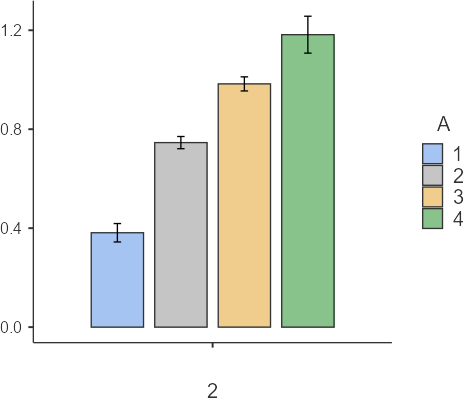
\includegraphics[width=\linewidth]{media/chem/image9}
\end{minipage} & 
\begin{minipage}[t]{\linewidth}
    \vspace{0pt} % Ensures proper alignment at the top
    \small{
    Солодка \\
    0.25 vs 0.5 \\
    p = 0.002 \\
    0.25 vs 0.75 \\
    0.25 vs 1.0 \\
    p < 0.001 \\
    0.5 vs 0.75 \\
    p = 0.026 \\
    0.5 vs 1.0 \\
    p < 0.001}
\end{minipage} & 
\begin{minipage}[t]{\linewidth}
    \vspace{0pt} % Ensures proper alignment at the top
    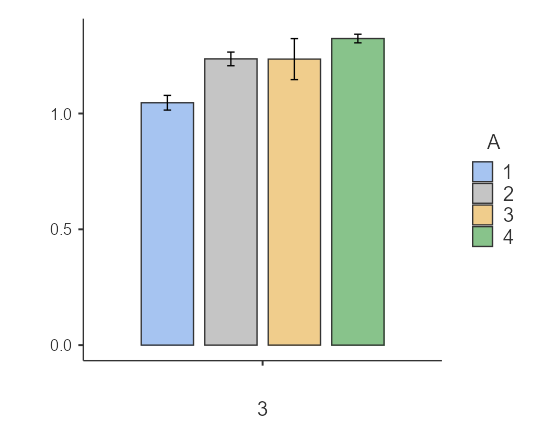
\includegraphics[width=\linewidth]{media/chem/image10}
\end{minipage} & 
\begin{minipage}[t]{\linewidth}
    \vspace{0pt} % Ensures proper alignment at the top
    \small{
    Хвощ \\
    0.25 vs 1.0 \\
    p = 0.019}
\end{minipage} \\
\begin{minipage}[t]{\linewidth}
    \vspace{0pt} % Ensures proper alignment at the top
    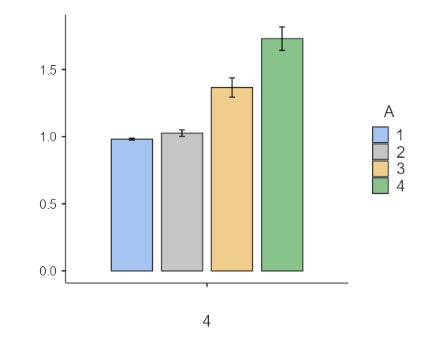
\includegraphics[width=\linewidth]{media/chem/image11}
\end{minipage} & 
\begin{minipage}[t]{\linewidth}
    \vspace{0pt} % Ensures proper alignment at the top
    \small{
    Одуванчик \\
    0.25 vs 0.75 \\
    p = 0.007 \\
    0.25 vs 1.0 \\
    p < 0.001 \\
    0.5 vs 0.75 \\
    p = 0.014 \\
    0.5 vs 1 \\
    p < 0.001 \\
    0.75 vs 1.0 \\
    p = 0.010}
\end{minipage} & 
\begin{minipage}[t]{\linewidth}
    \vspace{0pt} % Ensures proper alignment at the top
    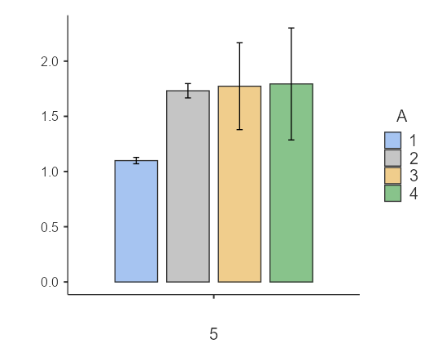
\includegraphics[width=\linewidth]{media/chem/image12}
\end{minipage} & 
\begin{minipage}[t]{\linewidth}
    \vspace{0pt} % Ensures proper alignment at the top
    \small{Гармала}
\end{minipage} \\
\end{tabular}
\begin{figure}[H]
\caption*{1 – 0.25 мг/мл, 2 – 0.5 мг/мл, 3 – 0.75 мг/мл, 4 – 1.0 мг/мл}
\caption*{Рис. 1 - Статистический метод: ANOVA с Tukey Post-Hoc Test
Доза-зависимый эффект}
\end{figure}

\begin{multicols}{2}
Для оценки АРА указанных объектов применен метод ингибирования DPPH
анализируемыми веществами.~ Антирадикальный эффект исследуемого объекта
проявляется в уменьшении оптической плотности раствора DPPH,
обусловленного переходом радикала DPPH в нерадикальную форму в
результате антирадикального действия исследуемого вещества. Показателем
антирадикального свойства в данной методике является величина АРА,
поэтому для объяснения механизма действия конкретного объекта необходимо
знание химической структуры соединения.~В таблице 4 приведены данные
исследования зависимости антирадикальной активности от концентрации
исследуемых образцов по отношению к ВНА. Изучение антирадикального
эффекта экстрактов выявило, что гармала обладает выраженной активностью,
однако ниже антиоксидантного эффекта ВНА, в свою очередь экстракты
солодки, хвоща и одуванчика проявляют активность ниже, чем вещество
стандарт, и с повышением концентрации активность соответственно
понижается.
\end{multicols}

\begin{table}[H]
\caption*{Таблица 4 - Зависимость АОА (\%) от концентрации растворов}
\centering
\begin{tabular}{|l|r|r|r|r|}
\hline
Экстракт & \multicolumn{1}{l|}{0,25 мг/мл} & \multicolumn{1}{l|}{0,5 мг/мл} & \multicolumn{1}{l|}{0,75 мг/мл} & \multicolumn{1}{l|}{1 мг/мл} \\ \hline
Солодка (Glycyrrhiza glabra L.)       & 65,9 & 67,8 & 66,3 & 63,5 \\ \hline
Хвощ (Equisétum arvense L.)           & 62,8 & 61,7 & 52,2 & 41,3 \\ \hline
Одуванчик (Taroxacum officinale Wigg) & 72,5 & 72,8 & 71,2 & 71,5 \\ \hline
Гармала (Péganum hármala L.)          & 73,2 & 79,7 & 80,4 & 75,4 \\ \hline
ВНА                                   & 83,7 & 81,3 & 80,9 & 80,7 \\ \hline
\end{tabular}
\end{table}

\begin{multicols}{2}
{\bfseries Выводы.}

1. Установлено, что наибольшее содержание полифенольных соединений по
эквиваленту галловой кислоты имеет место с незначительной долей в
экстрактах Солодки и Одуванчика, поэтому эти объекты можно рекомендовать
для дальнейшего изучения на биологическую активность \emph{in vivo}.

2. FRAP-методом определено, что по сравнению с Солодкой наибольшим
потенциалом обладает экстракт Гармалы.

3. Изучение антирадикального эффекта экстрактов выявило, что Гармала
обладает выраженной активностью, однако ниже антиоксидантного эффекта
ВНА.

На основе полученных данных мы считаем, что экстракты указанных видов
растений могут найти применение в качестве антиоксидантов и представляют
интерес для изучения антирадикальной активности и антиоксидантного
действия \emph{in vivo}.
\end{multicols}

\begin{center}
{\bfseries Литература}
\end{center}

\begin{references}
1. Adom, M. B., Taher, M., Mutalabisin, M. F., Amri, M. S., Abdul Kudos,
M. B., Wan Sulaiman, M. W. A.,Susanti, D. Chemical constituents and
medical benefits of Plantago major // Biomedicine \& Pharmaco-therapy.
- 2017. --Vol. 96. --P. 348--360. DOI: 10.1016/j.biopha.2017.09.152

2. Нукебай, А.К. Применение экстрактов, выделенных из корней солодки
голой (Glycyrrhiza glabra L.) // Молодой ученый. - 2021. - № 18 (360).
- С. 75-77. URL: https://moluch.ru/archive/360/80637

3. Nile S.H., Keum Y.S., Nile A.S., Jalde S.S., Patel R.V. Antioxidant,
anti-inflammatory, and enzyme inhibitory activity of natural plant
flavonoids and their synthesized derivatives // J. Biochem. Mol.
Toxicol. 2018. V. 32. № 1. DOI 10.1002/jbt.22002

4. K. Paulpriya, M. Packia Lincy, P.S. Tresina, V.R. Mohan. In vitro
Antioxidant Activity, Total Phenolic and Total Flavonoid Contents of
Aerial Part Extracts of Daphnipfyllum neilgherrense (WT) Rosenth // J.
Bio. Innov.- 2015. --Vol. 4(6). - P. 257-268.

5. Адекенова А.С., Тулеуова Г.Х., Hohmann J., Адекенов С.М.
Фармакогностическое изучение сырья Chartolepis intermedia Boiss. и
Peganum harmala L. // Известия НАН РК. Серия биологическая и
медицинская. - 2016. - № 2(314). - С. 200-204.

6. Ботиров Э.Ж., Боначева В.М., Коломиц Н.Э. Химический состав и
биологическая активность метаболитов растений рода EQUISETUM L //
Химия растительного сырья. -- 2021. - № 1. -С. 5--26. DOI:
10.14258/jcprm.2021017760.

7. Теселкин Ю.О., Бабенкова И.В., Какорин П.А. Антиоксидантная активность
биологически активных веществ водных извлечений караганы гривастой
(Caragana Jubata (Pall.) // Сборник научных трудов съезда биофизиков
России: в 2 томах, том 2. - Краснодар, 2019. - С. 262-263.

8. Grauso L., De Falco B., Lanzotti V., Motti R. Stinging nettle, Urtica
dioica L.: botanical, phytochemical and pharmacological overview //
Phytochemistry Reviews. -- 2020. -Vol. 19. -P. 1341--1377.
\\DOI:10.1007/s11101-020-09680-x

9. Иванова А.В., Газизуллина Е.Р., Попова К.Г., Матерн А.И. Исследование
антиоксидантной активности и суммарного содержания полифенолов
лекарственного растительного сырья // Журн. аналит. химии. - 2017. -Т.
72. -№ 4. -С. 363-368. DOI: 10.7868/S0044450217040053

10. Николаева Т.Н., Лапшин П.В., Загоскина Н.В. Метод определения
суммарного соедржания в растительных экстрактах с реактивом
Фолина-Дениса и реактивом Фолина-Чокальтеу: модификация и сравнение //
Химия растительного сырья. -- 2021. - № 2. - С. 291-299. DOI:
10.14258/jcprm.2021028250

11. Казбекова А.Т., Атажанова Г.А., Сейтембетов Т.С., Сейтембетова А.Ж.,
Болатов А.К., Адекенов С.М. Оценка антиоксидантной и антирадикальной
активности \emph{in vitro} экстрактов растений Казахстана//Вестник
ЗКГМУ им. М. Оспанова.-2017.- №1. -- С. 233-235.

12. Sapiyeva A.O., Kazbekova A.Т., Madiyeva Sh.A., Kenzheshova A.K.,
Baysarov G.M., Seytembetov T.S., Adekenov S. M. Correlation of
indicators of independent methods for determining the antioxidant
activity of bioflavonoids//International Multidisciplinary Medical
Science Journal. -2020.-Vol.1 -№1. -Р.14-20.
Stinging nettle, Urtica dioica L.: botanical, phytochemical
and pharmacological overview
\end{references}

\begin{center}
{\bfseries References}
\end{center}


\begin{references}
1. Adom, M. B., Taher, M., Mutalabisin, M. F., Amri, M. S., Abdul Kudos,
M. B., Wan Sulaiman, M. W. A.,Susanti, D. Chemical constituents and
medical benefits of Plantago major // Biomedicine \& Pharmaco-therapy.
- 2017. --Vol. 96. --P. 348--360. DOI 10.1016/j.biopha.2017.09.152

2. Nukebai, A.K. Primenenie ekstraktov, vydelennykh iz kornei solodki
goloi (Glycyrrhiza glabra L.) // Molodoi uchenyi. - 2021. - № 18
(360). - S. 75-77. URL: https://moluch.ru/archive/360/80637 {[}in
Russian{]}

3. Nile S.H., Keum Y.S., Nile A.S., Jalde S.S., Patel R.V. Antioxidant,
anti-inflammatory, and enzyme inhibitory activity of natural plant
flavonoids and their synthesized derivatives // J. Biochem. Mol.
Toxicol. 2018. V. 32. № 1. DOI 10.1002/jbt.22002

4. K. Paulpriya, M. Packia Lincy, P.S. Tresina, V.R. Mohan. In vitro
Antioxidant Activity, Total Phenolic and Total Flavonoid Contents of
Aerial Part Extracts of Daphnipfyllum neilgherrense (WT) Rosenth // J.
Bio. Innov.- 2015. --Vol. 4(6). - P. 257-268.

5. Adekenova A.S., Tuleuova G.Kh., Hohmann J., Adekenov S.M.
Farmakognosticheskoe izuchenie syr' ya Chartolepis
intermedia Boiss. i Peganum harmala L. // Izvestiya NAN RK. Seriya
biologicheskaya i meditsinskaya. - 2016. - № 2(314). - S. 200-204.
{[}in Russian{]}

6. Botirov E.Zh., Bonacheva V.M., Kolomits N.E. Khimicheskii sostav i
biologicheskaya aktivnost'{}\\ metabolitov rastenii roda
EQUISETUM L // Khimiya rastitel' nogo
syr' ya. -2021. -№ 1. -S. 5--26. DOI:
\\10.14258/jcprm.2021017760 {[}in Russian{]}

7. Teselkin Yu.O., Babenkova I.V., Kakorin P.A. Antioksidantnaya
aktivnost'{} biologicheski aktivnykh veshchestv vodnykh
izvlechenii karagany grivastoi (Caragana Jubata (Pall.) // Sbornik
nauchnykh trudov s"ezda biofizikov Rossii: v 2 tomakh, tom 2. -
Krasnodar, 2019. - S. 262-263. {[}in Russian{]}

8. Grauso L., De Falco B., Lanzotti V., Motti R. Stinging nettle, Urtica
dioica L.: botanical, phytochemical and pharmacological overview //
Phytochemistry Reviews, 2020, vol. 19, pp. 1341--1377.
\\DOI:10.1007/s11101-020-09680-x

9. Ivanova A.V., Gazizullina E.R., Popova K.G., Matern A.I. Issledovanie
antioksidantnoi aktivnosti i summarnogo soderzhaniya polifenolov
lekarstvennogo rastitel' nogo syr' ya //
Zhurn. analit. khimii. - 2017. -T. 72. -№ 4. -S. 363-368. DOI:
10.7868/S0044450217040053 {[}in Russian{]}

10. Nikolaeva T.N., Lapshin P.V., Zagoskina N.V. Metod opredeleniya
summarnogo soedrzhaniya v rastitel' nykh ekstraktakh s
reaktivom Folina-Denisa i reaktivom Folina-Chokal' teu:
modifikatsiya i sravnenie // Khimiya rastitel' nogo
syr' ya. -- 2021. - № 2. - S. 291-299. DOI:
10.14258/jcprm.2021028250 {[}in Russian{]}

11. Kazbekova A.T., Atazhanova G.A., Seitembetov T.S., Seitembetova A.Zh.,
Bolatov A.K., Adekenov S.M. Otsenka antioksidantnoi i
antiradikal' noi aktivnosti in vitro ekstraktov
rastenii Kazakhstana//Vestnik ZKGMU im. M. Ospanova.-2017.- №1. -- S.
233-235. {[}in Russian{]}

12. Sapiyeva A.O., Kazbekova A.Т., Madiyeva Sh.A., Kenzheshova A.K.,
Baysarov G.M., Seytembetov T.S., Adekenov S. M. Correlation of
indicators of independent methods for determining the antioxidant
activity of bioflavonoids//International Multidisciplinary Medical
Science Journal. -2020.-Vol.1 -№1. -Р.14-20.
\end{references}

\begin{authorinfo}
\hspace{1em}\emph{{\bfseries Сведения об авторах}}

Сапиева А.О. -кандидат химических наук, доцент, НАО «Медицинский
университет Астана», Астана, Казахстан, e-mail:
\href{mailto:sapieva.a@amu.kz}{\nolinkurl{sapieva.a@amu.kz}};

Мурзагалиева М.Г. - кандидат химических наук, ассоциированный профессор,
Алматы, Казахстан, e-mail:
\\\href{mailto:m_murzagalieva@mail.ru}{\nolinkurl{m\_murzagalieva@mail.ru}};

Ашимхан Н.С. - кандидат химических наук, ассоциированный профессор,
Алматы, Казахстан, e-mail:
\\\href{mailto:nazgul.ashimkhan@mail.ru}{\nolinkurl{nazgul.ashimkhan@mail.ru}};

Зейнульдина А.С.- кандидат химических наук, доцент, Астана, Казахстан,
e-mail:
\href{mailto:zeinuldina.a@amu.kz}{\nolinkurl{zeinuldina.a@amu.kz}};

Габбасова А.М. - кандидат химических наук, доцент, Астана, Казахстан,
e-mail:
\href{mailto:gabbasova.a@amu.kz}{\nolinkurl{gabbasova.a@amu.kz}};

Мадиева Ш.А.- магистр агрохимии и почвоведения, старший
преподаватель,Астана, Казахстан, e-mail:\\
\href{mailto:sharapat.828486@gmail.com}{\nolinkurl{sharapat.828486@gmail.com}};

Дюсекеева С.Б. -- магистр технических наук, старший преподаватель
кафедры общей и биологической химии, НАО «Медицинский университет
Астана», Астана, Казахстан, e-mail:
\href{mailto:dyussekeyeva.s@amu.kz}{\nolinkurl{dyussekeyeva.s@amu.kz}}.

\hspace{1em}\emph{{\bfseries Information about authors}}

Sapiyeva A. - Candidate of Chemical Sciences, Docent, Astana,
Kazakhstan, e-mail:
\href{mailto:sapieva.a@amu.kz}{\nolinkurl{sapieva.a@amu.kz}};

Murzagaliyeva M. - Candidate of Chemical Sciences, Associate Professor,
Almaty, Kazakhstan, e-mail:
\\\href{mailto:m_murzagalieva@mail.ru}{\nolinkurl{m\_murzagalieva@mail.ru}};

Ashimkhan N.- Candidate of Chemical Sciences, Associate Professor, ,
Almaty, Kazakhstan, e-mail:
\\\href{mailto:nazgul.ashimkhan@mail.ru}{\nolinkurl{nazgul.ashimkhan@mail.ru}};

Zeinuldina A. - Candidate of Chemical Sciences, Docent, Astana,
Kazakhstan, e-mail:
\href{mailto:zeinuldina.a@amu.kz}{\nolinkurl{zeinuldina.a@amu.kz}};

Gabbasova A. - Candidate of Chemical Sciences, Docent, Astana,
Kazakhstan, e-mail:
\href{mailto:gabbasova.a@amu.kz}{\nolinkurl{gabbasova.a@amu.kz}};

Madiyeva Sh.- Master of Agrochemistry and Soil Science, Senior
Lecturer,Astana, Kazakhstan, e-mail:\\
\href{mailto:sharapat.828486@gmail.com}{\nolinkurl{sharapat.828486@gmail.com}};

Dyussekeyeva S.- Master of Technical Sciences, Senior Lecturer, Astana,
Kazakhstan, e-mail:
\href{mailto:dyussekeyeva.s@amu.kz}{\nolinkurl{dyussekeyeva.s@amu.kz}}.
\end{authorinfo}
